The Engine for Likelihood-Free Inference (ELFI) \cite{1708.00707} is a
Python software library dedicated to likelihood-free inference
(LFI). ELFI models in a convenient manner all the fundamental
components of a Probabilistic Model such as priors, simulators,
summaries and distances. Furthermore, ELFI already supports a range of
likelihood-free inference methods proposed in the last years.

\subsubsection{Modelling}
\label{sec:modelling}

ELFI models the Probabilistic Model as a Directed Acyclic Graph (DAG);
it implements this functionality based on the package NetworkX, which
is designed for creating general purpose graphs. Although not
restricted to that, in most cases the structure of a likelihood-free
model follows the pattern presented in figure~\ref{fig:elfi-model};
there are edges that connect the \textit{prior} distributions to the
simulator, the simulator is connected to the summary statistics which
is turn are connected to the distance. The distance is the output
node. Samples can be obtained from all nodes through sequential
sampling. The nodes that are defined as
\textit{elfi.Prior}\footnote{The \textit{elfi.Prior} functionality is
  a wrapper around the scipy.stats package.} are automatically
considered as the parameters of interest and they are the only nodes
that, apart from sampling, they should also provide pdf
evaluation. The function passed as argument in the
\textit{elfi.Summary} node can be any valid Python function with
arguments the prior variables. Finally, the observations should be
passed in the appropriate node through the argument
\pinline{observed}; all the nodes afterwards are evaluated at the
observations as well.

\begin{figure}[!ht]
    \begin{center}
      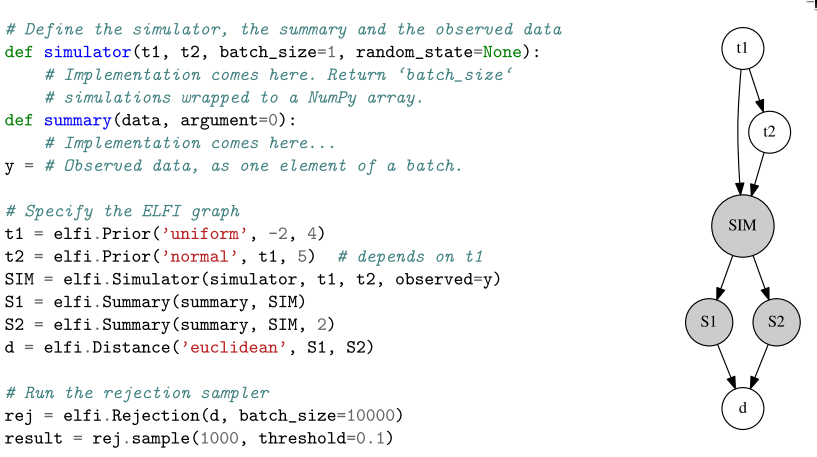
\includegraphics[width=0.8\textwidth]{./Thesis/images/chapter2/elfi.png}
    \end{center}
    \caption{Image taken from \cite{1708.00707}}
    \label{fig:elfi-model}
\end{figure}


\subsubsection{Inference Methods}
\label{sec:inference-methods}

The inference Methods implemented at the ELFI follow some common
guidelines; (a) the initial argument should be the output node
followed by the rest hyper-parameters of the method and (b) they must
provide a basic inference functionality, in most cases
$<$\textit{method}$>$\textit{.sample()} returning a predefined
\textit{elfi.Result} object containing the obtained samples along with
some other useful functionalities (e.g.\ plotting the marginal
posteriors).

The collection of likelihood-free inference methods implemented so far
contains the \textit{ABC Rejection Sampler} and \textit{Sequential
  Monte Carlo ABC Sampler}. A quite central method implemented by ELFI
is the \textit{Bayesian Optimisation for Likelihood-Free Inference
  (BOLFI)}, which is methodologically quite close to the ROMC method
that we implement in the current dissertation.

Add parallelisation ...


